% Euclidean Geometry Solutions
% Started in Summer 2020
\documentclass{tufte-handout}

%\geometry{showframe}% for debugging purposes -- displays the margins

%%%% Packages to make things pretty
\usepackage{amsmath,amsthm}
\usepackage{booktabs}
\usepackage{graphicx}
\setkeys{Gin}{width=\linewidth,totalheight=\textheight,keepaspectratio}
\graphicspath{{graphics/}}
\usepackage{units}
\usepackage{fancyvrb}
\fvset{fontsize=\normalsize}
\usepackage{multicol}
\usepackage{pdfpages}

%%%% Theorem Environments
\theoremstyle{definition}
\swapnumbers
\newtheorem{theorem}{Theorem}[section]
\newtheorem{definition}[theorem]{Definition}
\newtheorem{lemma}[theorem]{Lemma}
\newtheorem{corollary}[theorem]{Corollary}

%%%%%

\title[Solutions]{Solutions to Euclidean Geometry Tasks}
\author[Hitchman]{Theron J Hitchman}
\date{\today}

\begin{document}

\maketitle

\begin{marginfigure}
    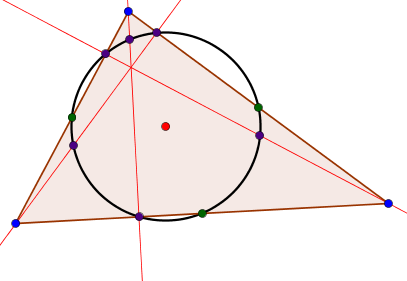
\includegraphics{images/NPC.png}
\end{marginfigure}

%%%% \setcounter{section}{-1}
\section*{Introduction}

I collect here solutions to the standard sequence of Euclidean Geometry tasks. As time goes on, I might add solutions devised by my students. For now I will just put down my favorite solution, without trying to figure out if it is one of mine, or one written by a student at some point in the last 12 years.

My thanks to all of my students, who have helped me to enjoy our time together doing mathematics by being clever, persistent, and open to learning new ways of thinking.

I'll do this section by section, but I won't necessarily do the tasks in order inside a given section. Instead, I will work through the material in a way that fits how I think about it. In particular, this means that the numbering of results here, given as [section].[item], will not necessarily match the numbering used in the notes. The section numbers will be the appropriate, but in each section the theorems might be proved in a different order. In fact, as one question or another might produce several different results as ``answers,'' the number of results generally does not match the number of questions.


\setcounter{section}{1}
\section{Beginnings: The Rhombus}\label{section:rhombi}

\begin{theorem}[Conjecture 1.1]\label{theorem:rhombus-opp-angles}
Let $ABCD$ be a rhombus. Then angle $ABC$ is congruent to angle $ADC$. Similarly, angle $BAD$ is congruent to angle $BCD$.
\end{theorem}

\begin{proof}
By Postulate 1, we may draw in the segment $AC$. This divides our rhombus into two triangles, triangle $ABC$ and triangle $ADC$.

\begin{marginfigure}
  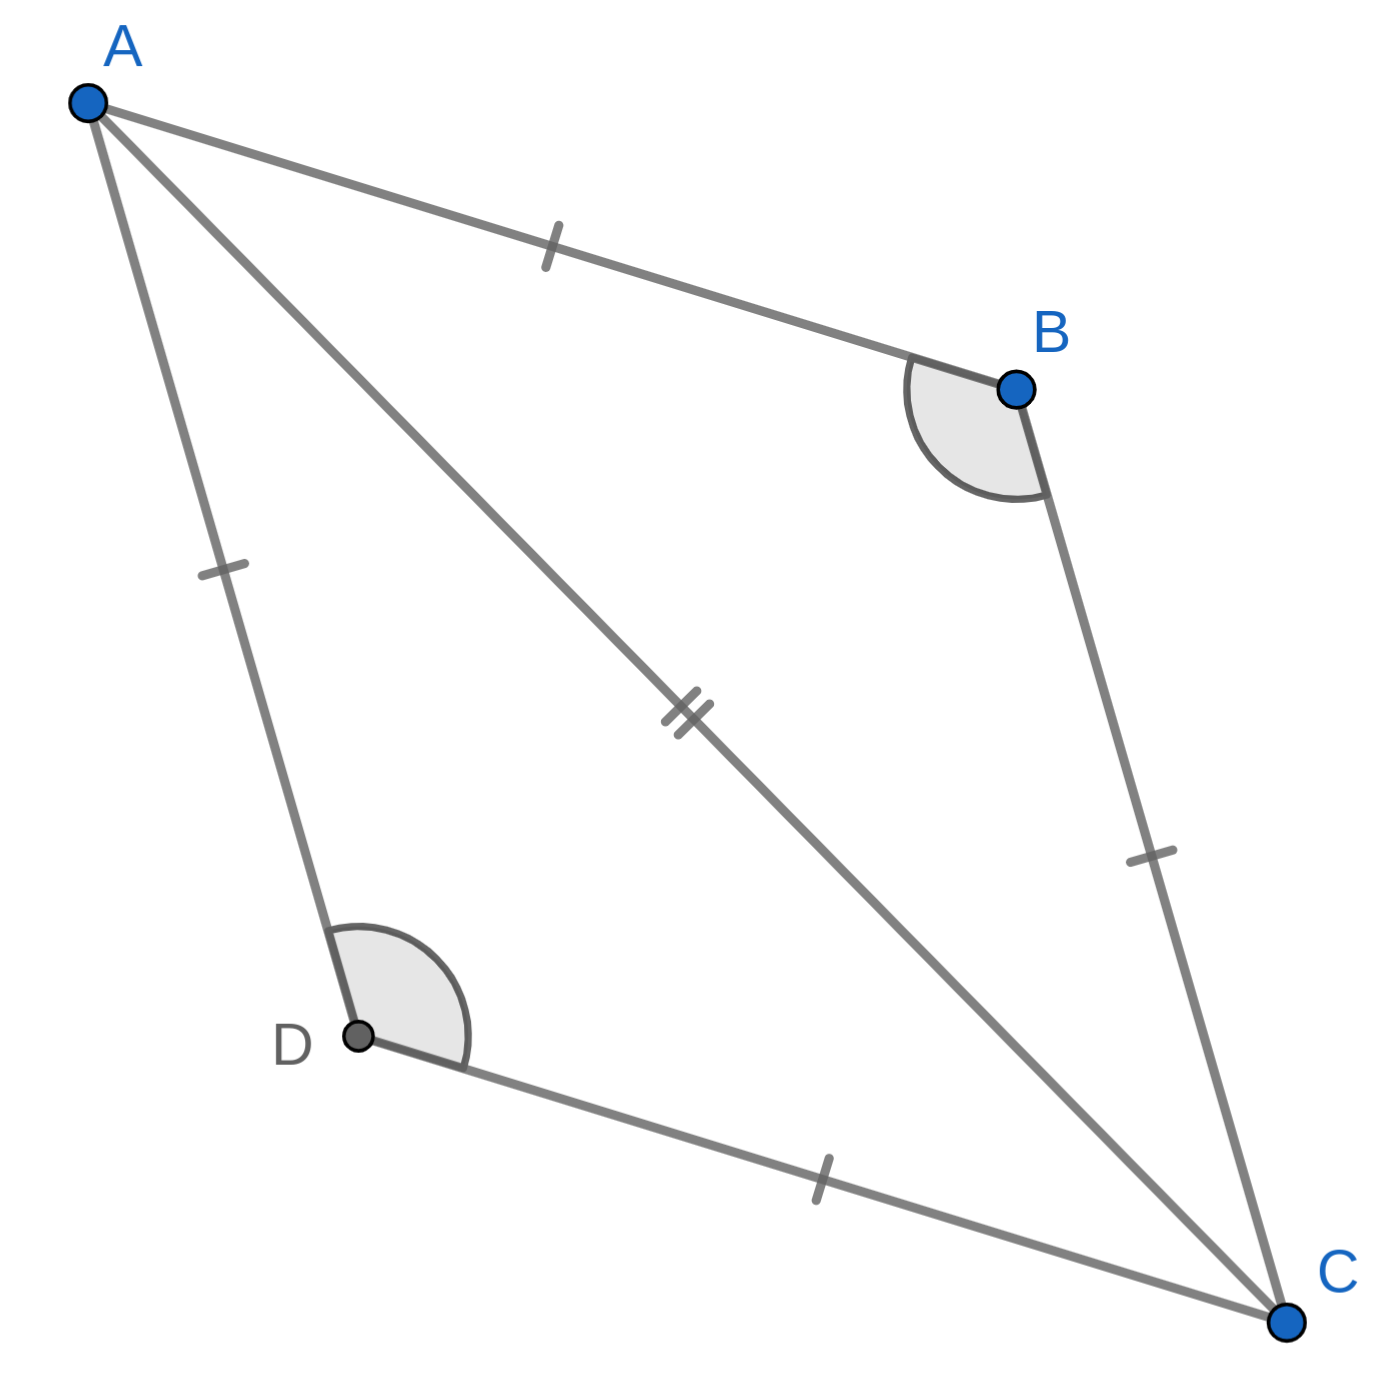
\includegraphics{images/rhombus_with_diagonal.png}
\end{marginfigure}

Since our original figure is a rhombus, we know that the four segments $AB$, $BC$, $CD$, and $DA$ are all congruent. In particular, $AB$ is congruent to $AD$ and $BC$ is congruent to $DC$. Also, the segment $AC$ is shared by both triangles and is congruent to itself. Therefore, by Euclid's proposition I.8, the two triangles $ABC$ and $ADC$ are congruent.

Since the two triangles are congruent, their corresponding angles are congruent, by the definition of congruent triangles. We conclude that angle $ABC$ is congruent to angle $ADC$.

We can obtain the second conclusion by entirely similar reasoning, but instead dividing the rhombus by the segment $BD$.
\end{proof}

\begin{corollary}\label{corollary:rhombus-angle-bisectors}
Let $ABCD$ be a rhombus. The diagonal $AC$ is an angle bisector for both angle $BAD$ and angle $BCD$.

Moreover, the diagonal $AC$ divides the rhombus into a pair of congruent isosceles triangles, with base angles sitting on the diagonal.
\end{corollary}

\begin{proof}
As in the proof of the theorem, we know that the triangles $ABC$ and $ADC$ are congruent. But since $ABCD$ is a rhombus, we also know that these triangles are isosceles. Since all four sides of the rhombus are congruent, we know that $AB$ is congruent to $BC$ and $AD$ is congruent to $DC$.

\begin{marginfigure}
  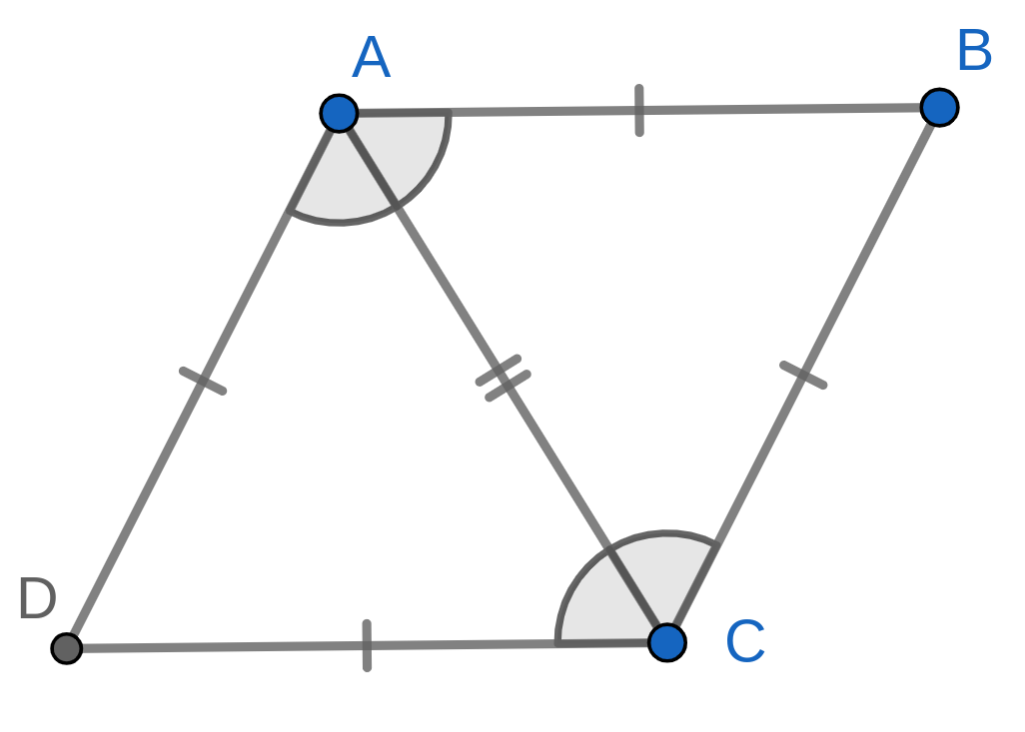
\includegraphics{images/rhombus_diagonal_marked.png}
\end{marginfigure}

So by Eulid's Proposition I.5, we conclude that the angles
$BAC$ and $BCA$ are congruent. The same holds for the angles $DAC$ and $DCA$. But these pairs of angles can be made to correspond to each other in the triangle congruence between triangle $ABC$ and triangle $ADC$. Therefore, all four of these angles must be congruent.

In particular, this means that the ray $AC$ cuts the angle $BAD$ into two congruent pieces: angle $BAC$ and angle $DAC$. Thus, $AC$ is the angle bisector of angle $BAD$. Similarly, $AC$ is the angle bisector of angle $BCD$.
\end{proof}

\begin{lemma}\label{lemma:rhombus-equilateral-triangles}
The three angles of an equilateral triangle are mutually congruent. Further, those angles are each congruent to two thirds of a right angle.
\end{lemma}

\begin{proof}
Let $ABC$ be an equilateral triangle. Since $AB$ is congruent to $AC$, by Euclid's Proposition I.5 angle $ABC$ is congruent to angle $ACB = BCA$.

Also, similarly since $BC$ is congruent to $BA$, by Proposition I.5 angle $BCA$ is congruent to angle $BAC = CAB$.

By a common notion,\sidenote{We won't quote common notions anymore after this.} all three of the angles $ABC$, $BCA$ and $CAB$ are congruent. By Euclid's Proposition I.32, these three angles taken together make two right angles. Therefore, each of these angles is congruent to two thirds of a right angle.
\end{proof}

\clearpage

\begin{theorem}[Conjecture 1.1]\label{theorem:rhombus-not-square}
There is a rhombus $ABCD$ such that angle $BAC$ and $BDC$ are not congruent.
\end{theorem}

\begin{proof}
We shall construct such a rhombus directly. The idea is to use the method of construction in Euclid's Proposition I.1.

Pick a pair of points $A$ and $C$. Use Postulate 3 to construct circles $AC$ and $CA$. By the Circle-Circle Intersection Property,\sidenote{This is an extra axiom discussed in the introductory notes given to students.} these two circles meet at two points. We call these two points $B$ and $D$. Finally, join up these points with Postulate 1 to form segments $AB$, $BC$, $CD$, and $DA$. By the argument in Euclid's Proposition I.1, this figure $ABCD$ is a rhombus.

\begin{marginfigure}
  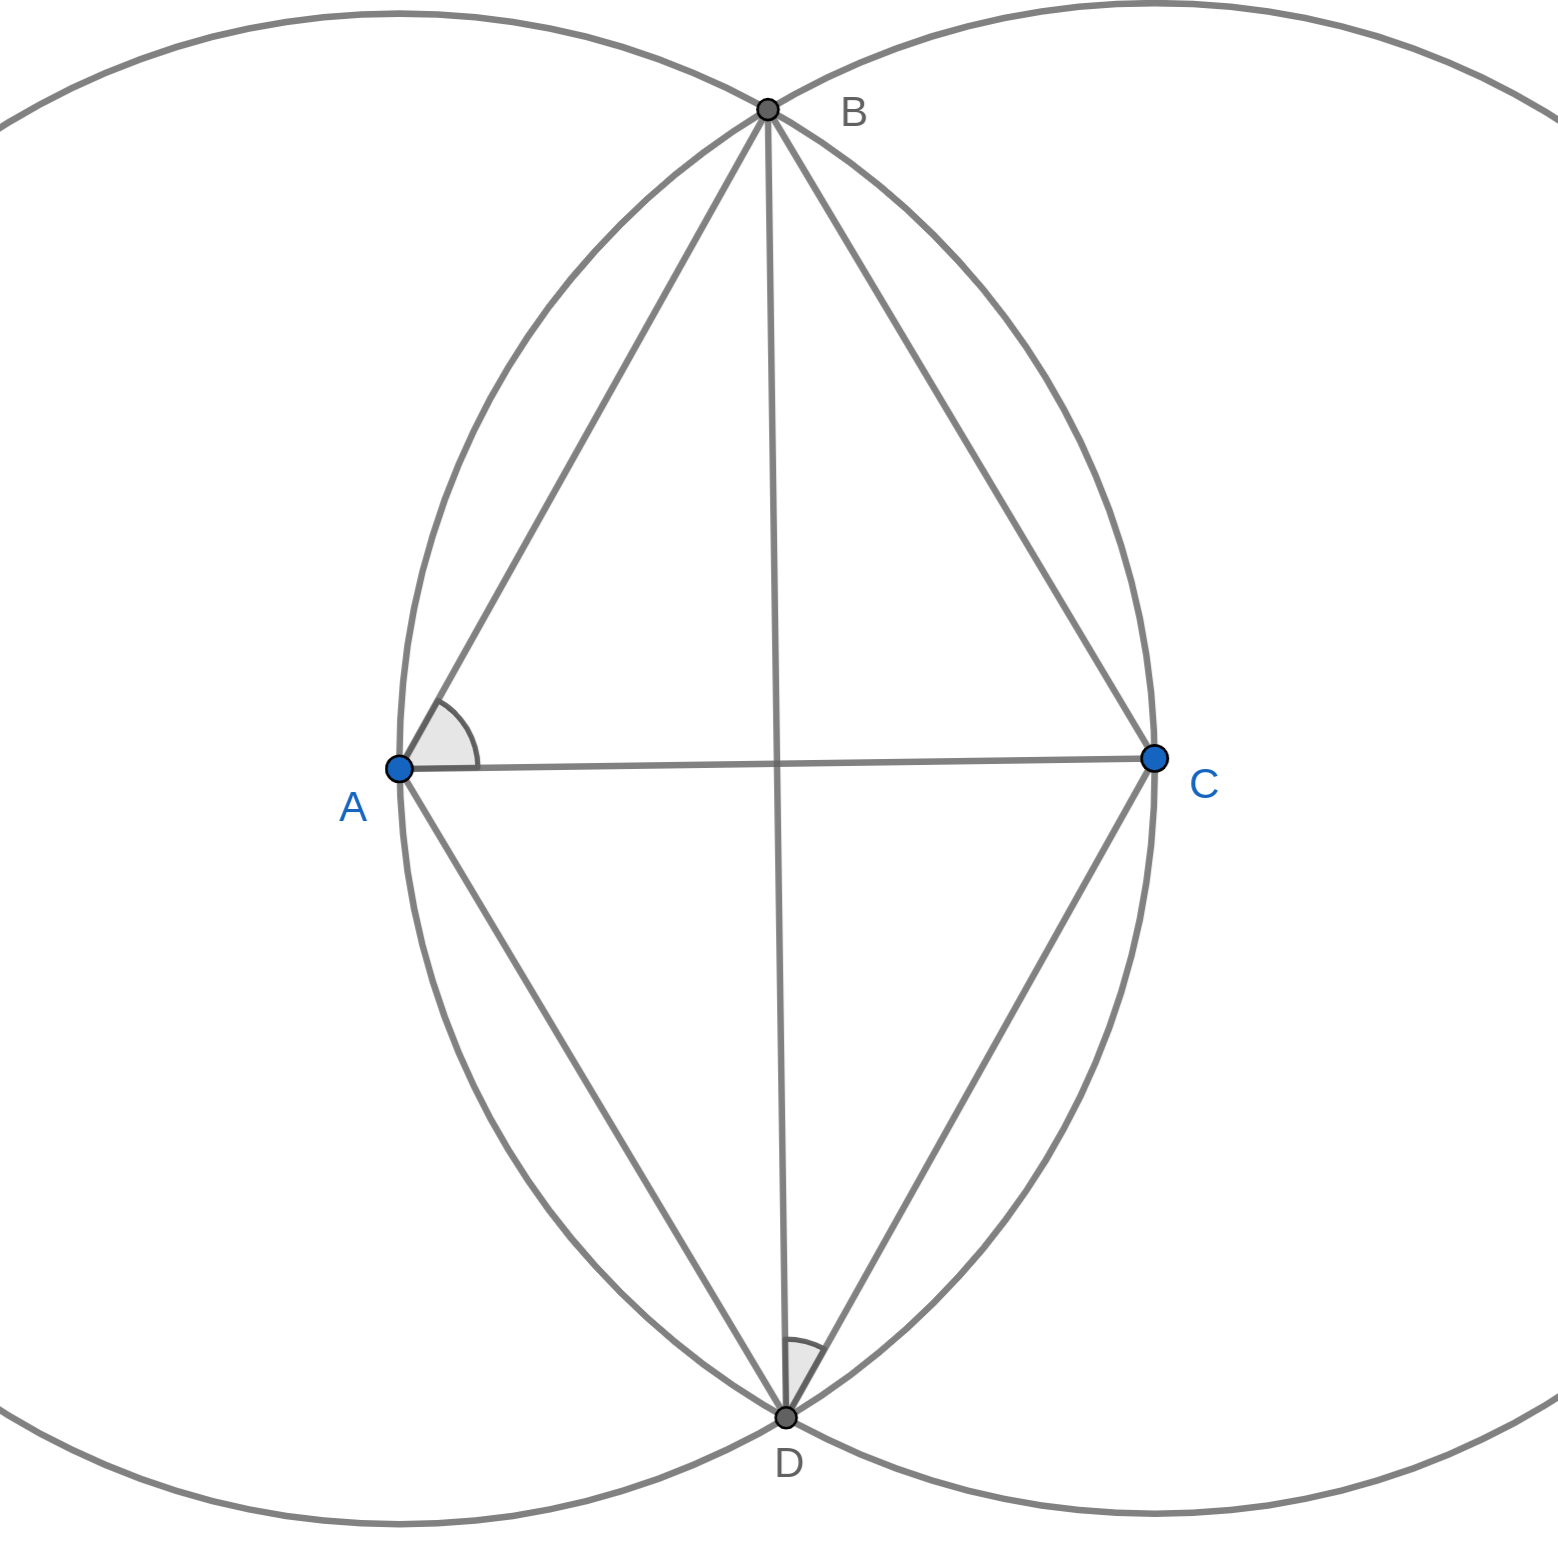
\includegraphics{images/double_equilateral.png}
\end{marginfigure}

However, we have built an interesting and special rhombus, made of two equilateral triangles with a shared side. The angle $BAC$ is one of the angles in one of these equilateral triangles.

Now draw segment $BD$ by Postulate 2. Note that angle $BDC$ is only part of angle $ADC$, so by a common notion $BDC$ is less than $ADC$. Note that angle $ADC$ is one of the angles in one of the equilateral triangles. So angle $ADC$ is congruent to angle $BAC$.

If we put these together, we see that angle $BDC$ is less than angle $BAC$. Thus these two angles are not congruent.
\end{proof}

\begin{theorem}[Conjectures 1.4 \& 1.5]\label{theorem:rhombus-construction}
Given a segment $AB$ and an angle $XYZ$, there exists a rhombus $ABCD$ with the angle at $A$ congruent to angle $XYZ$.
\end{theorem}

\begin{proof}
We will construct a rhombus directly. First, by Postulate 3 we may draw a circle $AB$, with center at $A$ and passing through $B$. By Postulates 2 and 1, in that order, draw the line through $A$ and $B$. By Euclid's Proposition I.23 we construct a ray $r$ with initial point $A$ so that this ray makes an angle with line $AB$ congruent to angle $XYZ$. Where $r$ meets the circle $AB$, mark the point $D$.

\begin{marginfigure}
  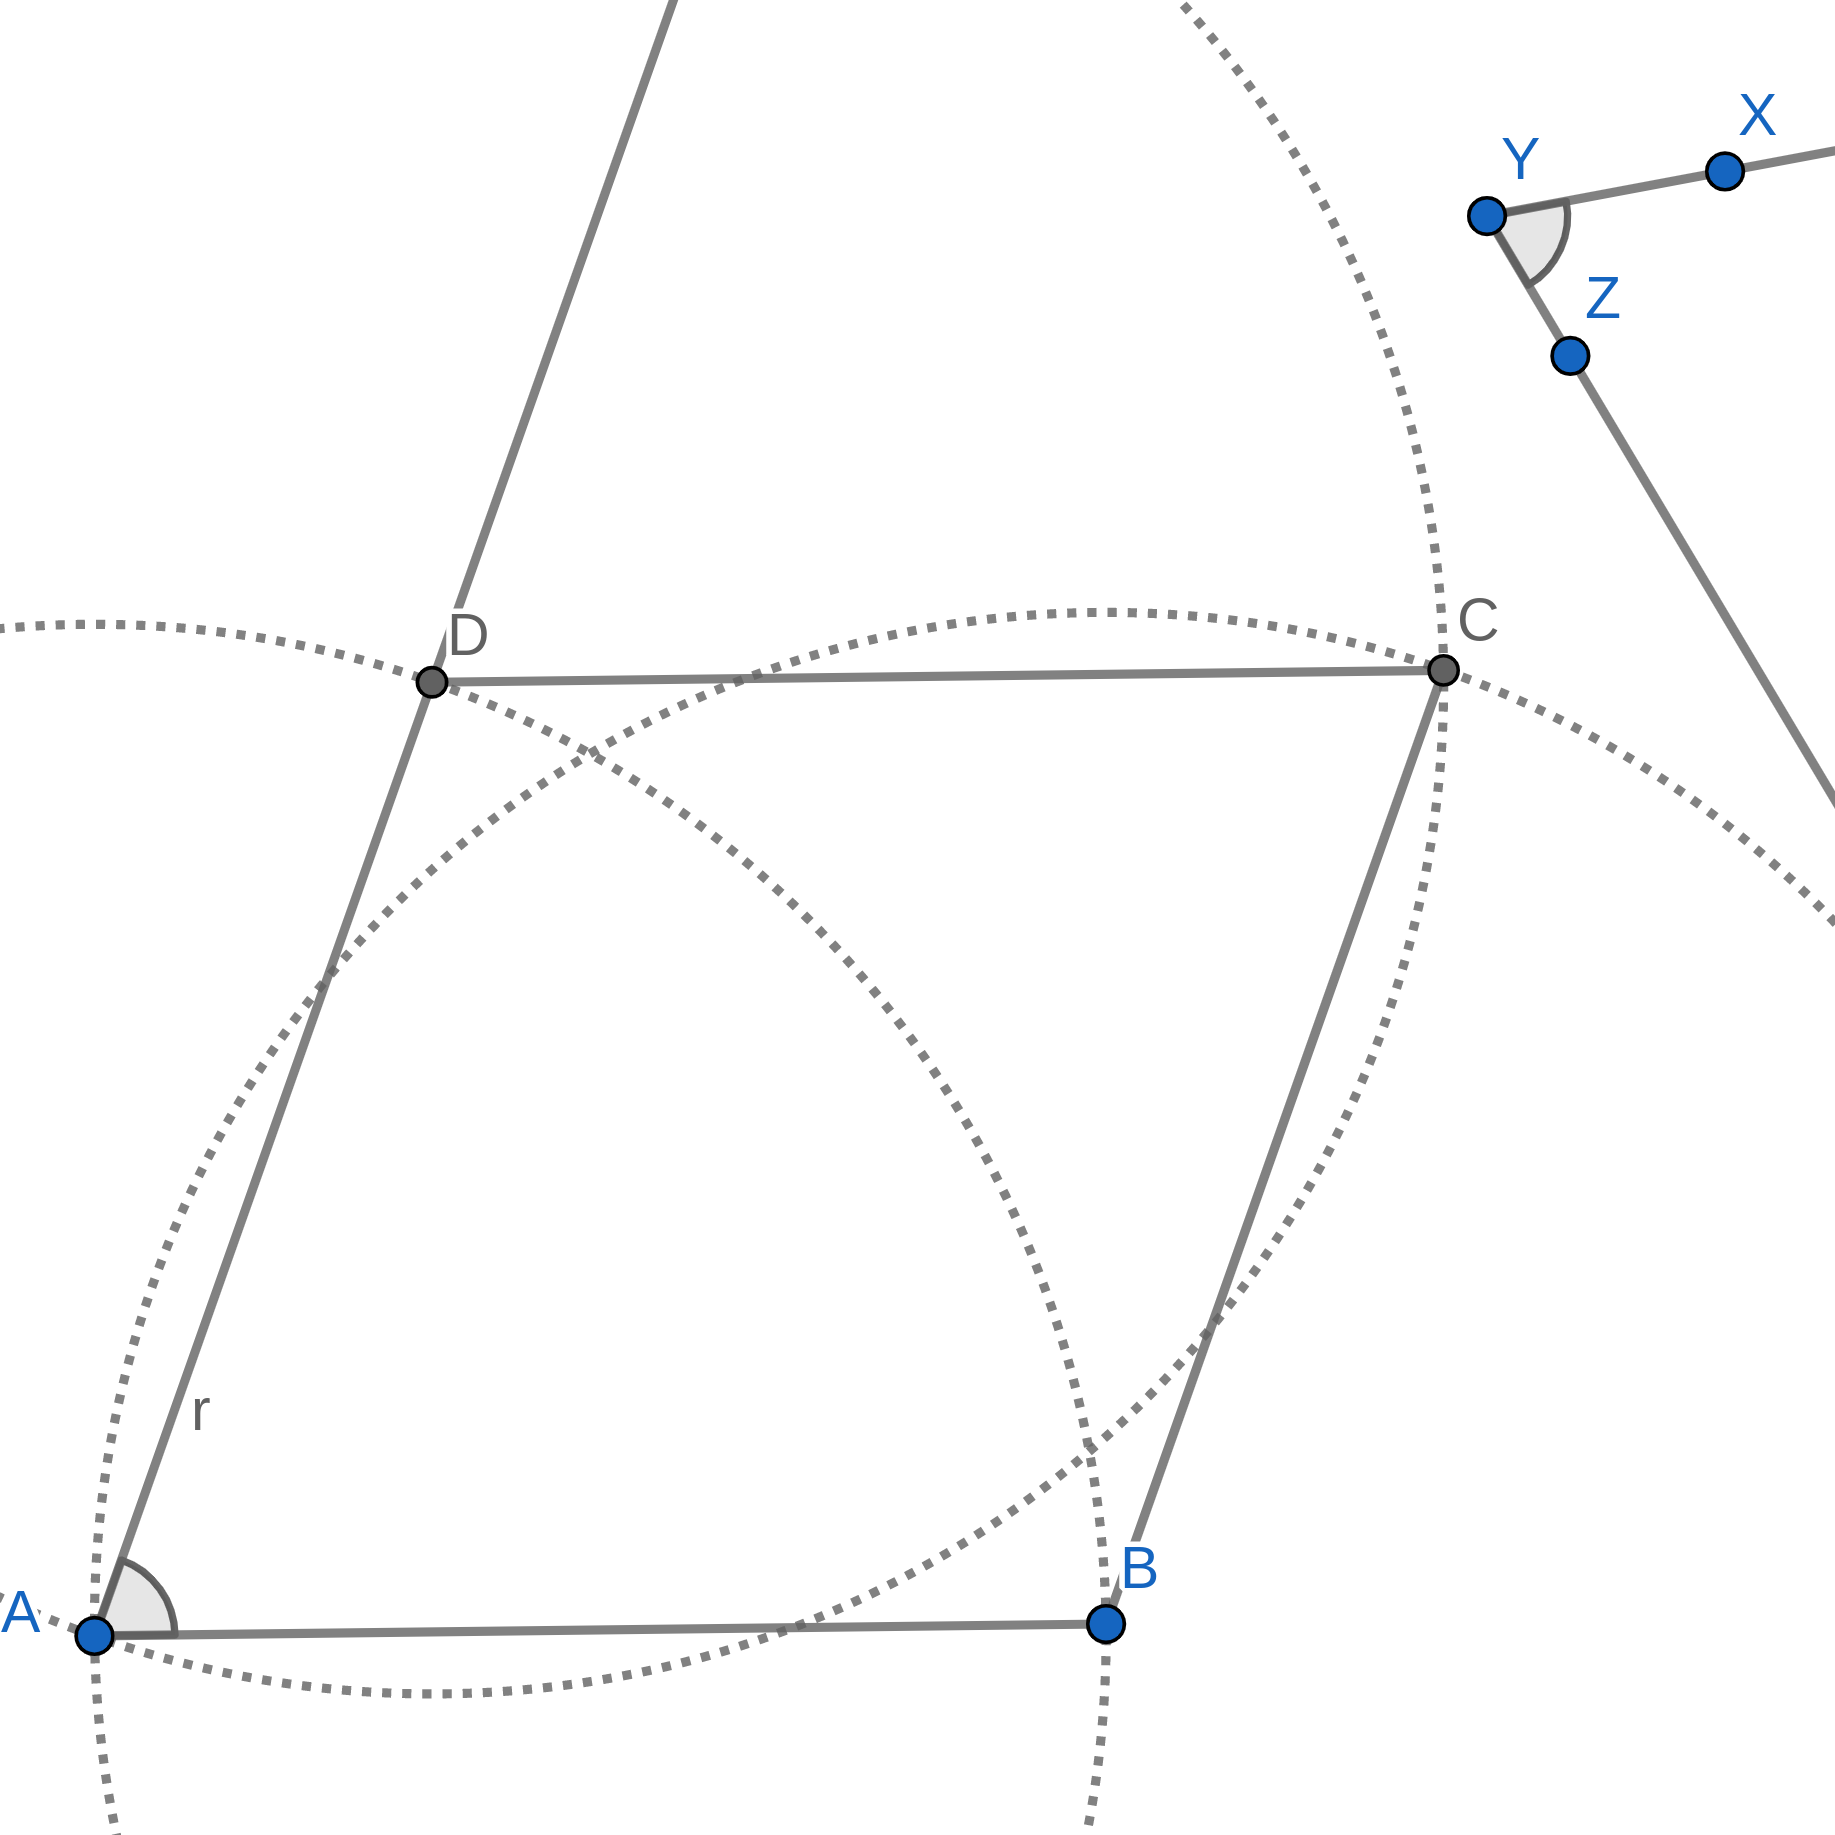
\includegraphics{images/rhombus_construction.png}
\end{marginfigure}


Now draw two more circles: circle $DA$ with center $D$ and passing through $A$ and circle $BA$ with center $B$ also passing through $A$. These two circles meet at $A$. By the Circle-Circle Intersection Property, they also meet at another point, which we call $C$.

Finally we draw the remaining required line segments to make the rhombus. By Postulate 2, we draw $BC$ and $CD$. We claim that the resulting quadrilateral $ABCD$ is the one required.

By construction, the angle $DAB$ is congruent to angle $XYZ$. Segments $AB$ and $AD$ are radii of the common circle $AB$, so they are congruent by the definition of a circle. Similar reasoning shows that $AD$ is congruent to $DC$, and $DC$ is congruent to $BC$. Therefore, all four sides of $ABCD$ are mutually congruent, and hence $ABCD$ is a rhombus.

\end{proof}



\begin{definition}[Parallelogram, inferred from Euclid I.33] \label{definition:parallelogram}
A quadrilateral $ABCD$ is a \emph{parallelogram} if for each pair of opposite segments, extending those segments to lines makes a pair of parallel lines.
\end{definition}


\begin{theorem}{Conjecture 1.6}\label{theorem:rhombus-parallelogram}
Suppose that $ABCD$ is a rhombus. Then $ABCD$ is a parallelogram.
\end{theorem}

\begin{proof}
Consider the rhombus $ABCD$, and extend the four sides to lines using Postulate 2. Also, by Postulates 1 and 2, draw the line $AC$ containing the diagonal segment $AC$. We will show that the lines $AB$ and $CD$ are parallel.

\begin{marginfigure}
  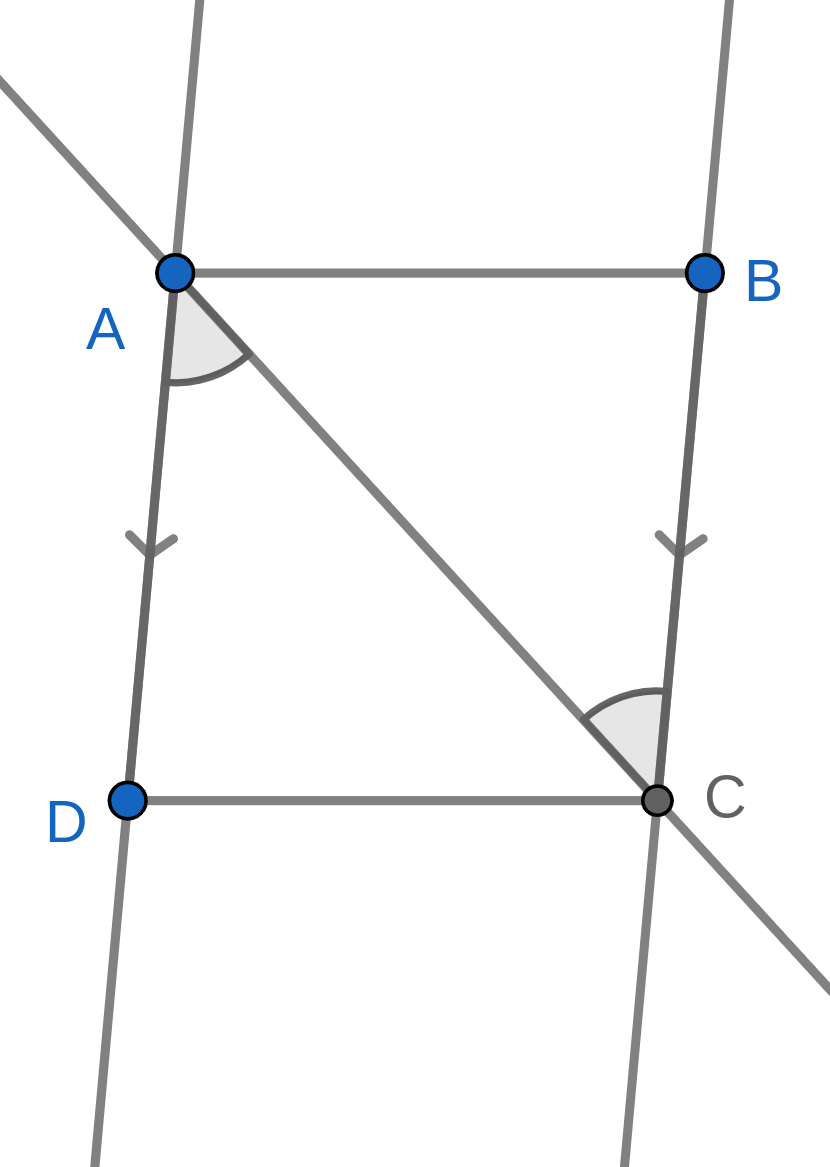
\includegraphics{images/rhombus_parallel_sides.png}
\end{marginfigure}

By Corollary \ref{corollary:rhombus-angle-bisectors}, we see that $AC$ divides the rhombus into a pair of congruent isosceles triangles: triangle $ABC$ and triangle $ADC$. We conclude that angle $BCA$ is congruent to angle $DAC$.

This means that the line $AC$ falls upon the lines $AB$ and $CD$ in such a way as to make the alternate interior angles congruent. By Euclid's Proposition I.27, the lines $AB$ and $CD$ are parallel.

One argues for the other pair of sides in an entirely similar manner, but using angles $BAC$ and $ACD$ instead.
\end{proof}


\begin{corollary}[Conjecture 1.1]\label{corollary:rhombus-rigidity}
Let $ABCD$ be a rhombus. If angle $BAC$ is congruent to angle $BDC$, then $ABCD$ is a square.
\end{corollary}

\begin{proof}
By Corollary \ref{corollary:rhombus-angle-bisectors}, adding the diagonal $AC$ divides the rhombus $ABCD$ into a pair of congruent isosceles triangles $ABC$ and $ADC$. In particular, the angles $BAC$ and $CAD$ are congruent.

The same argument works for dividing the rhombus with the diagonal $BD$, and we learn that angles $BDA$ and $BDC$ are congruent.

\begin{marginfigure}
  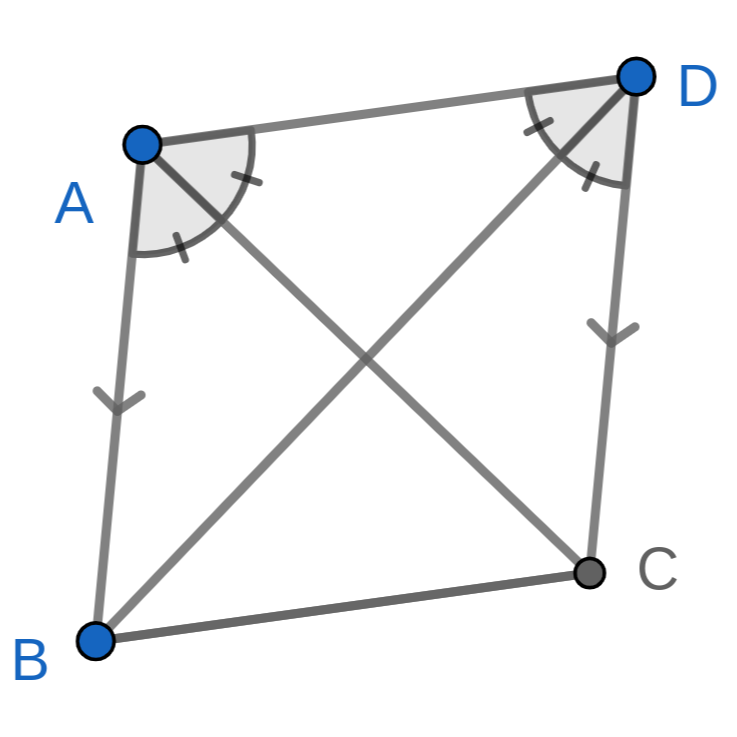
\includegraphics{images/rhombus_rigidity.png}
\end{marginfigure}

By our hypothesis, this means that all four of the angles $BAC$, $ACD$, $BDA$, and $BDC$ are congruent. Gathering these together in pairs which share a side, and using the fact that sums of equals must be equal, we see that angle $BAD$ is congruent to angle $ADC$.

But since $ABCD$ is a parallelogram, the lines $AB$ and $DC$ are parallel. Note that the line $AD$ falls upon them with the angles $BAD$ and $ADC$ being the pair of interior angles on the same side. So by Euclid's Proposition I.29, these angles taken together make two right angles. Since they are congruent and together make two right angles, each must be a right angle.

Looking closer, we see that each of the angles $BAC$, $ACD$, $BDA$, and $BDC$ is congruent to half a right angle.
By Euclid's proposition I.5, the same must be true for the angles $BCA$, $ACD$, $ABD$, and $DBC$. Gathering these together in pairs which share a side, we learn that angles $ABC$ and $BCD$ are right angles.

Since $ABCD$ is a quadrilateral having four mutually congruent sides and four right angles, it is a square.
\end{proof}


\begin{theorem}[Conjecture 1.7]\label{theorem:rhombus-diags-perp}
Let $ABCD$ be a rhombus, if the segments $AC$ and $BD$ meet at a point $X$, then $AXB$ is a right angle.\sidenote{One can get more out of this: namely the two diagonals divide the rhombus into four right triangles which are all mutually congruent.}
\end{theorem}

\begin{proof}
Let $ABCD$ be a rhombus for which the segments $AC$ and $BD$ meet at a point $X$. Consider the two triangles $AXB$ and $AXD$. We want to show that these triangles are congruent.

\begin{marginfigure}
  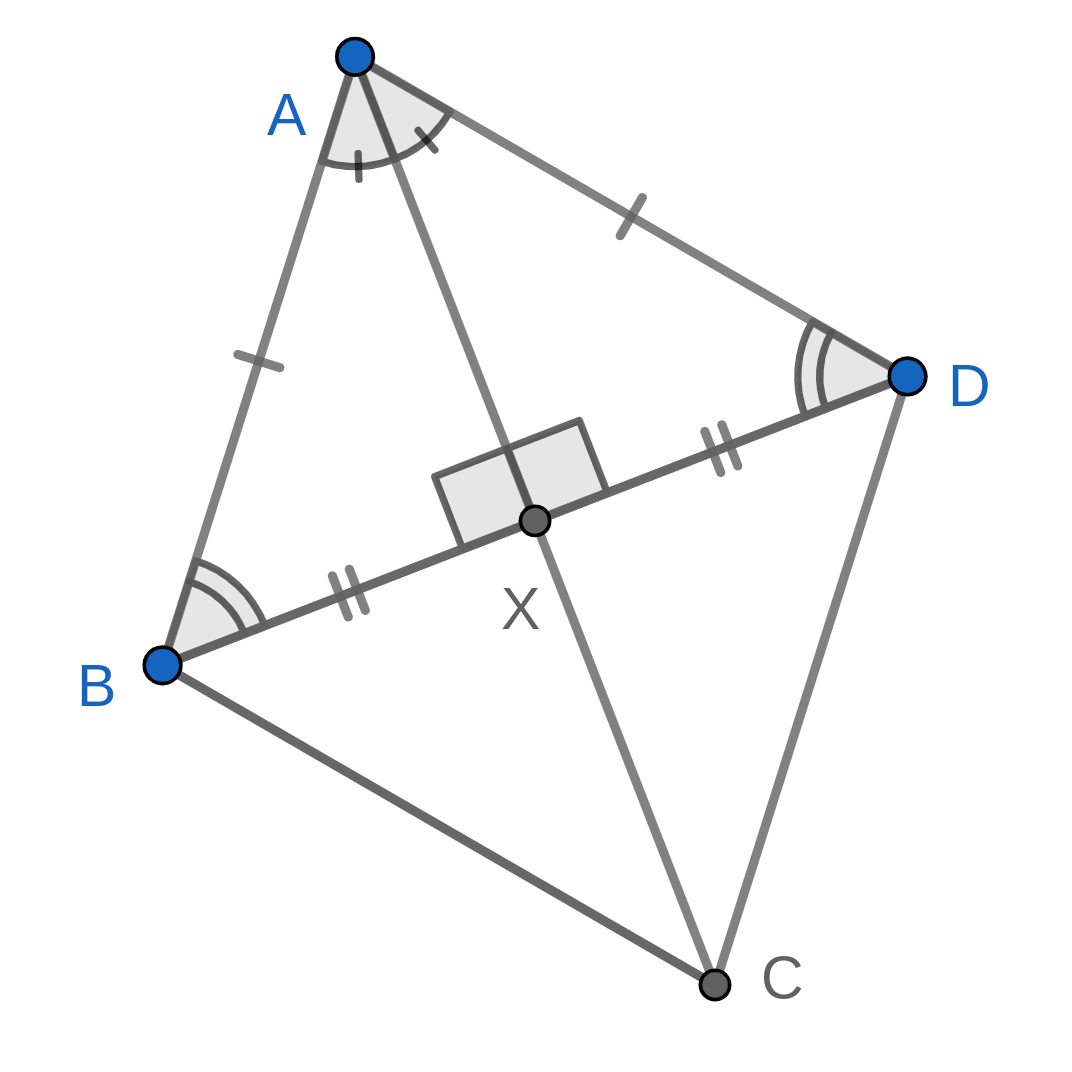
\includegraphics{images/rhombus_diags_perp.png}
\end{marginfigure}

Since $ABCD$ is a rhombus, the segments $AB$ and $AD$ are congruent. We deduce that triangle $BAD$ is isosceles and hence that angle $XBA = DBA$ is congruent to angle $XDA = BDA$ by Euclid's Proposition I.5. By Corollary \ref{corollary:rhombus-angle-bisectors} $AC$ is an angle bisector of angle $BAD$, so angle $BAX$ is congruent to angle $DAX$. So by Euclid's Proposition I.26, triangle $AXB$ is congruent to triangle $AXD$.

In this pair of congruent triangles, the angles $AXB$ and $AXD$ correspond. Also, these two angles are formed by the inclination of the line $AC$ through the line $BD$ at the point $X$, so by Euclid Proposition I.13, these angles either are two right angles, or taken together make as much as two right angles. As these angles are equal, we see that each must be a right angle. In particular, $AXB$ is a right angle.
\end{proof}



\begin{theorem}[Conjecture 1.2]\label{theorem:rhombus-diags-meet}
Let $ABCD$ be a rhombus. Then the diagonal segments $AC$ and $BD$ intersect.
\end{theorem}

\begin{proof}
We have seen that $ABCD$ is necessarily a parallelogram, so by Euclid's Proposition I.29, the angles $BAD$ and $CDA$ taken together make two right angles. We have proved that the diagonal $AC$ is the angle bisector of angle $BAD$ and the diagonal $BD$ is the angle bisector of angle $CDA$. Therefore, the angles $CAD$ and $BDA$ taken together are half of two right angles, which is certainly less than two right angles.

\begin{marginfigure}[-0.75in]
  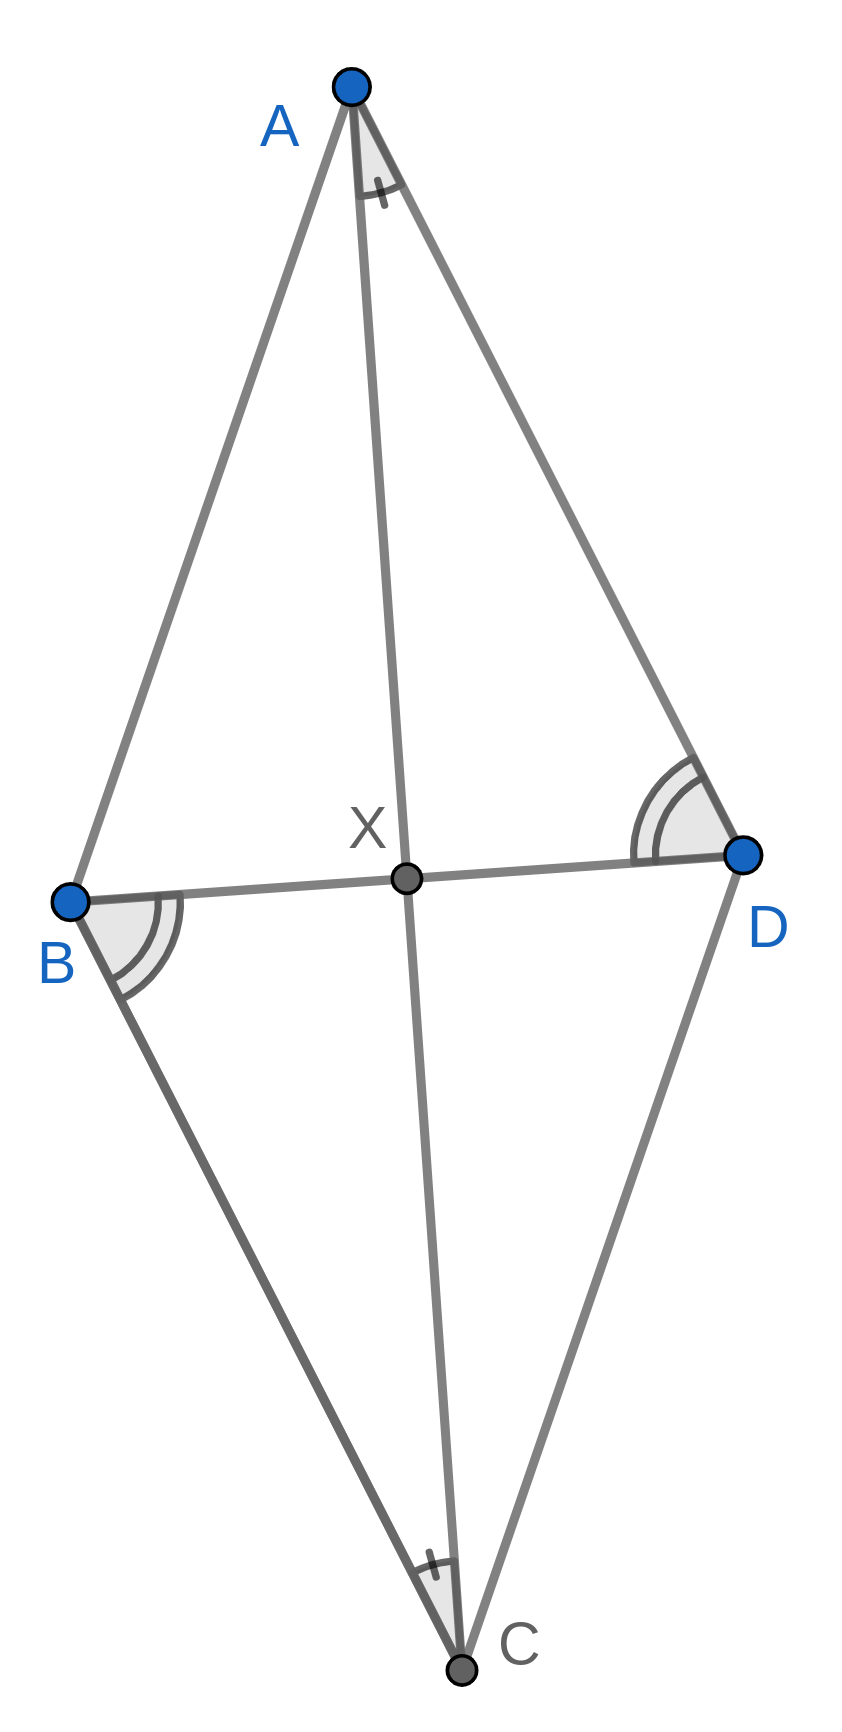
\includegraphics{images/rhombus_diag_meet.png}
\end{marginfigure}

So, by Euclid's Postulate 5, the rays $AC$ and $BD$ meet at some point $X$. By the statement of Postulate 5, $A$ does not lie between $C$ and $X$ in line $AC$. Similarly, $B$ does not lie between $D$ and $X$ on line $BD$.\sidenote{One set of axioms which is needed but appears only implicitly in Euclid's work is a collection of ideas and methods for dealing with \emph{between-ness}. In this case, we need the notion of what it means for one point on a line to lie between two other points on that line.}

Let's repeat the argument, but now working at the vertices on the opposite side $BD$. Following the same arguments, we see that the rays $CA$ and $DB$ meet at some point $Y$, which is situated so that $C$ does not separate $A$ and $Y$ in line $AC$ and $D$ does not separate $B$ and $Y$ in $BD$.

Now, the two lines $AC$ and $BD$ are different, so they can meet only once.\sidenote{Here is another unnoticed axiom!} This means that $X$ and $Y$ are the same point. Also, we learn that $X$ lies between $A$ and $C$ on line $AC$, and hence in the \emph{segment} $AC$. Similarly $X$ lies in the \emph{segment} $BD$.

We deduce that the diagonal segments $AC$ and $BD$ intersect.
\end{proof}

\clearpage

\begin{proof}[Alternate Proof of Theorem \ref{theorem:rhombus-diags-meet}]
Consider the rhombus $ABCD$ with diagonal $BD$. By Euclid's Proposition I.10, we may construct the midpoint $M$ of segment $BD$, so that $BM$ is congruent to $MD$. We shall first show that the triangles $ABM$ and $ADM$ are congruent.

\begin{marginfigure}
  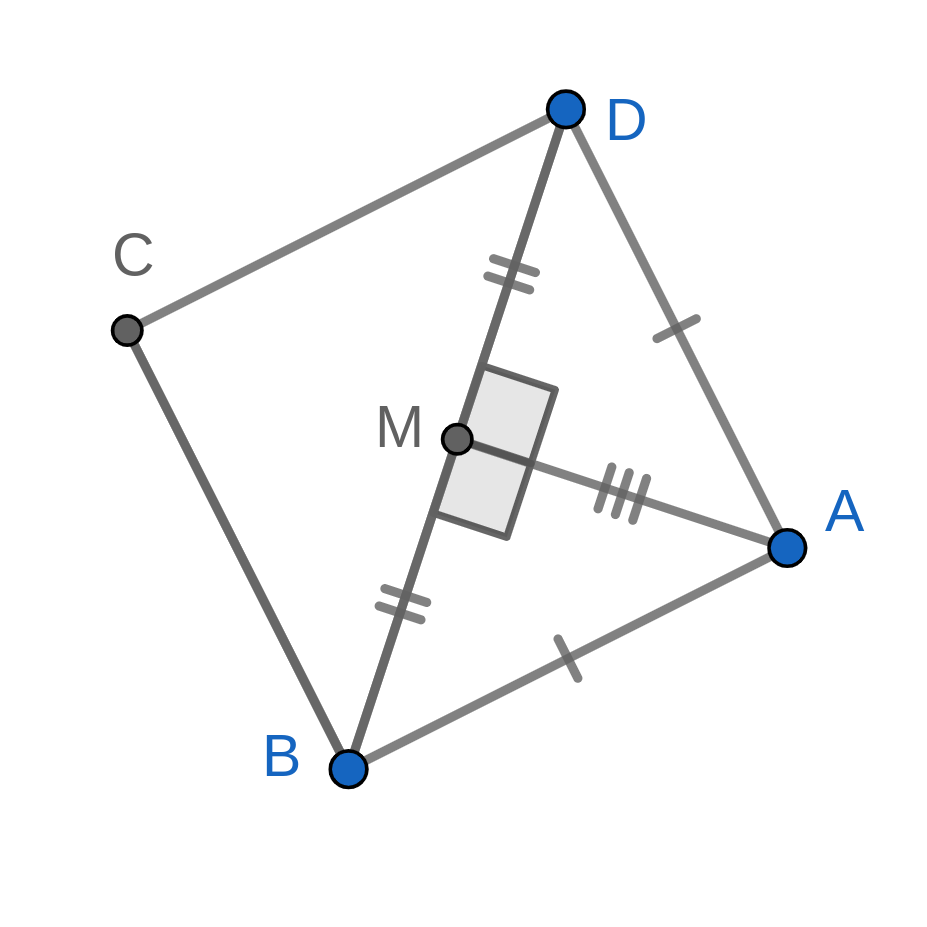
\includegraphics{images/rhombus_midpt_diag_pf.png}
\end{marginfigure}

Note that since $ABCD$ is a rhombus, the segments $AB$ and $AD$ are congruent. By construction of the point $M$, the segments $BM$ and $DM$ are congruent. Finally, the segment $MA$ is common to both triangles, and is congruent to itself. So by Euclid's Proposition I.8, the triangles $ABM$ and $ADM$ are congruent.

Since corresponding parts of congruent triangles are congruent, we deduce that angle $BMA$ is congruent to angle $DMA$. But these angles are the result of the straight line $AM$ being set up on the straight line $BD$, so by Euclid's Proposition I.13 these angles must either be two right angles, or taken together must make as much as two right angles. Since our angles are congruent, they must each be a right angle.

We can make exactly the same arguments as above with the triangles $CBM$ and $DBM$. We deduce that the angles $DMC$ and $BMC$ are also right angles.

We are now in the situation of Euclid's Proposition I.14, where the two lines $AM$ and $CM$ lie on opposite sides of the line $BD$, and make angles which taken together make two right angles. We conclude that $AM$ and $CM$ are parts of a single line. This means that $A$, $M$ and $C$ are collinear.

Now we know that the segment $AC$ meets the segment $BD$ at the midpoint $M$ of $BD$. In particular, these segments intersect.
\end{proof}



\setcounter{section}{2}
\setcounter{theorem}{0}
\section{The Kite}\label{section:kites}


\begin{theorem}\label{theorem:kites-1}
here is a thing about kites
\end{theorem}







\end{document}


